\documentclass{article}
\usepackage{tikz}
\usetikzlibrary{shapes.geometric}

\begin{document}
    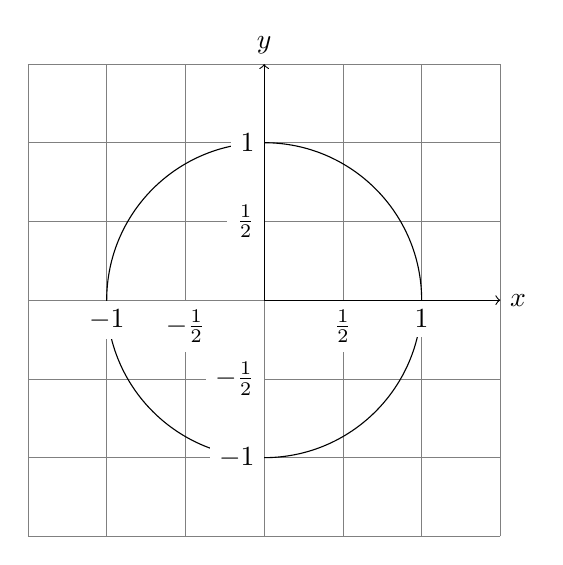
\begin{tikzpicture}
        \draw[help lines] (-3,-3) grid(3,3);
        \draw[->] (0,0) --(0,3) node[above]{$y$};
        \draw[->] (0,0) --(3,0) node[right]{$x$};
        \draw[] (0,0) circle(2);
        \node[below, fill=white]at(-1,0){$-\frac{1}{2}$};
        \node[below, fill=white]at(-2,0){$-1$};
        \node[left, fill=white]at(0,1){$\frac{1}{2}$};
        \node[left, fill=white]at(0,2){$1$};
        \node[below, fill=white]at(1,0){$\frac{1}{2}$};
        \node[below, fill=white]at(2,0){$1$};
        \node[left, fill=white]at(0,-1){$-\frac{1}{2}$};
        \node[left, fill=white]at(0,-2){$-1$};
    \end{tikzpicture}

    \newpage
    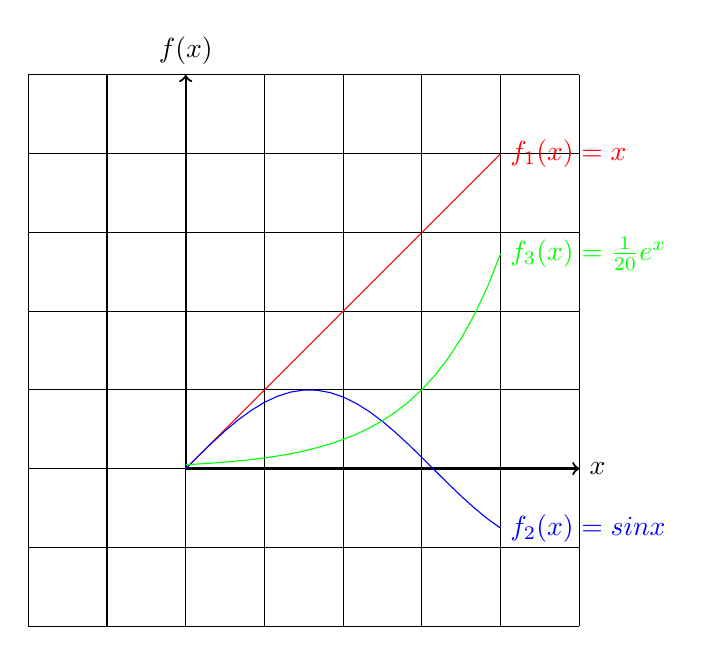
\begin{tikzpicture}
        \draw[] (-2,-2) grid(5,5);
        \draw[->, thick] (0,0) --(0,5) node[above]{$f(x)$};
        \draw[->, thick] (0,0) --(5,0) node[right]{$x$};
        \draw[domain=0:4, red] (0,0) plot(\x, {\x}) node[right]{$f_1(x)=x$};
        \draw[domain=0:4, blue] (0,0) plot(\x, {sin(\x r)}) node[right]{$f_2(x)=sin x$};
        \draw[domain=0:4, green] (0,0) plot(\x, {0.05*exp(\x)}) node[right]{$f_3(x)=\frac{1}{20}e^x$};
    \end{tikzpicture}

    \vspace{7mm}
    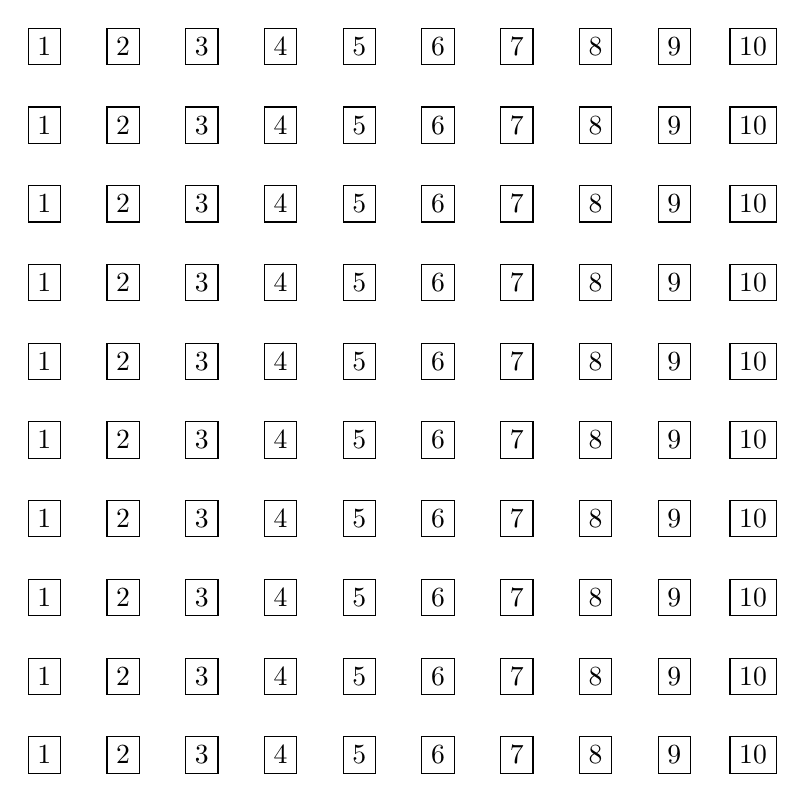
\begin{tikzpicture}
        \foreach \x in {1,...,10}
        {
            \foreach \y in {1,...,10}
            {
                \node[draw, rectangle]at(\x, \y){\x};
            }
        }
    \end{tikzpicture}

    \newpage
    \begin{tikzpicture}
        \tikzstyle{every node}=[draw, circle, green, text=black]

        \node[](1){1}
            [sibling distance=4cm, level distance=1.3cm]
            child{
                node[](2){2} edge from parent[->]
                child{
                    node[](4){4} edge from parent[->]
                }
                child{
                    node[](5){5} edge from parent[->]
                }
            }
            child{
                node[](3){3} edge from parent[->]
            };

        \node[](10)at(6,0){10};
        \node[](11)at(8,0){11};
        \draw[->] (10) ..controls(6.5,1)and(7.5,1).. (11);
        \draw[->] (11) ..controls(7.5,-1)and(6.5,-1).. (10);
    \end{tikzpicture}
\end{document}
